% !TeX spellcheck = en_US
% !TeX encoding = utf8
% !TeX program = xelatex
% !BIB program = bibtex

\documentclass[12pt]{article}
	\usepackage{amsmath,amssymb,amsfonts}
	\usepackage{hyperref}
	\usepackage{latexsym}
	\usepackage{graphicx}
	\usepackage{verbatim}
	\usepackage{booktabs}
	\usepackage[usenames,dvipsnames,svgnames,table]{xcolor}
	\usepackage{todonotes} % Required for the boxes that questions appear in
	\usepackage{mmstyles}
	\newcommand{\mybox}[1]
	{
	\par\noindent
	\todo[inline, backgroundcolor=SkyBlue!40,bordercolor=SkyBlue,size=\large]{\textbf{#1}}
	
	}

	\usepackage[top=25mm, bottom=25mm, left=18mm, right=18mm]{geometry}

	\usepackage{fancyhdr}
	\pagestyle{fancy}
	\lhead{Linear Optimization Assignment \#3}
	\chead{}
	\rhead{Due: Friday, May 4}
	\renewcommand{\headrulewidth}{0.3pt}

	% \usepackage[framed,numbered,autolinebreaks,useliterate,final]{mcode}
	\usepackage{listings}
	\title{\textbf{Linear Optimization Assignment \#3}}
	\author{Due: Friday, May 4}
	\date{}

	% \makeatletter
	% \def\@seccntformat#1{%
	% 	\expandafter\ifx\csname c@#1\endcsname\c@section\else
	% 	\csname the#1\endcsname\quad
	% 	\fi}
	% \makeatother

	\usepackage{multirow}
	\usepackage{sectsty}
	\usepackage{fontspec}
	\usepackage[slantfont,boldfont]{xeCJK}
	% \sectionfont{\color{NavyBlue}\selectfont}
	% \subsectionfont{\color{SkyBlue}\itshape\selectfont}

	\newcommand{\abs}[1]{\left| #1 \right| }
	\newcommand{\norm}[1]{\left\| {#1} \right\|}
	\newcommand{\red}[1]{{\color{red}{#1}}}
	\usepackage{titlesec,titletoc} 
	\renewcommand*{\thesection}{\color{NavyBlue}Problem \arabic{section} } 
	\renewcommand*{\thesubsection}{\color{SkyBlue}Solution \arabic{section} } 
	\titleformat{\section}[hang]{\bfseries}{\thesection}{1em}{}{}
	\titleformat{\subsection}[hang]{\itshape}{\thesubsection}{1em}{}{}
	
	% \setlength{\parsep}{0em}
	% \setlength{\itemsep}{0pt}
	\setlength{\parskip}{.33em}
	\setlength{\parindent}{0em}	

	\providecommand{\tightlist}{%
	\setlength{\itemsep}{0pt}\setlength{\parskip}{0pt}}
  
\begin{document}
% \vspace{-1em}
\maketitle

\textbf{\color{NavyBlue}Instruction:} Write a report and complete code.
Download the code from ftp (10.13.71.168). Upload report and code to ftp (10.13.72.84) or send email to 907682447@qq.com.
\begin{itemize}
	\tightlist
	\item {Please} name the report as \red{hw3\_31xxxxxxxx.pdf} and use pdf format; {Please} name the compressed file as \red{hw3\_31xxxxxxxx.zip} or \red{hw3\_31xxxxxxxx.rar}. And put our name and other information into report.
	\item Upload:
	      \begin{itemize}
		      \tightlist
		      \item    Address: 10.13.72.84
		      \item Username: opt; Passwd:  opt18; Port: 21
	      \end{itemize}
	\item Download:
	      \begin{itemize}
		      \tightlist
		      \item Address: 10.13.71.168
		      \item  Username: opt; Passwd:  opt18; Port: 21
	      \end{itemize}
\end{itemize}

% ------------------------------
\section{Convolution Arithmetic}

\begin{description}
	\item[(a)]
	      Assume we have a kernel matrix, with kernel size of $3$ along both vertical axis $i$ and horizontal axis $j$,
	      $$\mK = \begin{bmatrix}
			      0 & 1 & 2 \\
			      2 & 2 & 0 \\
			      0 & 1 & 2
		      \end{bmatrix}$$, and have a feature map, with input size of $5\times 5$
	      $$\mX =  \begin{bmatrix}
			      3 & 3 & 2 & 1 & 0 \\
			      0 & 0 & 1 & 3 & 1 \\
			      3 & 1 & 2 & 2 & 3 \\
			      2 & 0 & 0 & 2 & 2 \\
			      2 & 0 & 0 & 0 & 1
		      \end{bmatrix}$$
	      When this $3\times 3$ kernel is applied  to a $5 \times 5$ input padded with a $1 \times 1$ border of zeros using $2 \times 2$ strides, write down the output feature map of discrete convolution operation?
	\item[(b)] When a $k\times k$ kernel is applied  to a $i \times i$ input padded with a $p \times p$ border of zeros using $s \times s$ strides, write down the shape of output $o \times o$ feature map.

	      Assume $i_1+2p-k$ is a multiple of $s$, and the output shape is $o_1$, then is there any other input size $i_x$ to produce same $o_1$?

	      Hint: There is no ambiguity when $s=1$, but when $s\ge 2$, for example, if $i=10,k=3,s=2,p=1$, then $o$ is 5 rather than $11/2$. 
	\item[(c)] Apply 64 $5\times 5\times 3$ kernel to a $32 \times 32 \times3$ input with \red{unit stride and no padding, \ie using $1  \times 1$ strides and padding with a $0\times 0$ border of zeros}, how many float point operation do we need? (We only consider multiply operation, since it is more computational consuming than sum operation). \red{What about unit stride and same padding? \ie Using $1 \times 1$ strides and  padding with a $2 \times 2$ border of zeros?} 
	\item[(d)] The whole VGGNet is composed of CONV layers that perform 3x3 convolutions with stride 1 and pad 1, and of POOL layers that perform 2x2 max pooling with stride 2 (and no padding). We can write out the size of the representation at each step of the processing and keep track of both the representation size and the total number of weights. Let us fill in the blank:
	\begin{verbatim}
INPUT: [224x224x3]        memory:  224*224*3=150K   weights: 0
CONV3-64: [224x224x64]  memory:  224*224*64=3.2M   weights: (3*3*3)*64 = 1,728
CONV3-64: _______________  memory:  _______________   weights: _______________
POOL2: _______________  memory:  _______________   weights: _______________
CONV3-128: [112x112x128]  memory:  112*112*128=1.6M   weights: (3*3*64)*128 = 73,728
CONV3-128: [112x112x128]  memory:  112*112*128=1.6M   weights: (3*3*128)*128 = 147,456
POOL2: [56x56x128]  memory:  56*56*128=400K   weights: 0
CONV3-256: [56x56x256]  memory:  56*56*256=800K   weights: (3*3*128)*256 = 294,912
CONV3-256: [56x56x256]  memory:  56*56*256=800K   weights: (3*3*256)*256 = 589,824
CONV3-256: [56x56x256]  memory:  56*56*256=800K   weights: (3*3*256)*256 = 589,824
POOL2: [28x28x256]  memory:  28*28*256=200K   weights: 0
CONV3-512: [28x28x512]  memory:  28*28*512=400K   weights: (3*3*256)*512 = 1,179,648
CONV3-512: [28x28x512]  memory:  28*28*512=400K   weights: (3*3*512)*512 = 2,359,296
CONV3-512: [28x28x512]  memory:  28*28*512=400K   weights: (3*3*512)*512 = 2,359,296
POOL2: [14x14x512]  memory:  14*14*512=100K   weights: 0
CONV3-512: [14x14x512]  memory:  14*14*512=100K   weights: (3*3*512)*512 = 2,359,296
CONV3-512: [14x14x512]  memory:  14*14*512=100K   weights: (3*3*512)*512 = 2,359,296
CONV3-512: [14x14x512]  memory:  14*14*512=100K   weights: (3*3*512)*512 = 2,359,296
POOL2: [7x7x512]  memory:  7*7*512=25K  weights: 0
FC: [1x1x4096]  memory:  4096  weights: _______________
FC: [1x1x4096]  memory:  4096  weights: 4096*4096 = 16,777,216
FC: [1x1x1000]  memory:  1000 weights: 4096*1000 = 4,096,000
	\end{verbatim}

\end{description}

\subsection{Convolution Arithmetic} 

(a) 
$\begin{bmatrix}
		6 & 17 & 3 \\ 
		8& 17 & 13 \\ 
		6& 4&4 
	\end{bmatrix}$ 
(1 pnt) 过程 0.5 pnt

(b) 根据提示应该有有向下取整,$o=\lfloor (i-k+2p)/s \rfloor +1$,(2 pnts),若写成 $o= (i-k+2p)/s +1$,则1 pnts。 

$i_x = i_1 +1, i_1+2, ... ,i_1+s-1$ (1 pnt)

(c) 第一问 5x5x3x28x28x64=3763200 1 pnt, 第二问 5x5x3x32x32x64=4915200 0.5 pnt. 

(d) 每空0.5 pnt,一共3.5 pnts

\begin{figure}[h]
	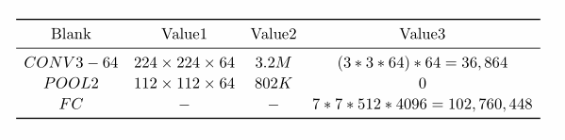
\includegraphics[width=.8\textwidth]{fig/2018-05-03-21-10-02.png}
\end{figure}

\section{Convolution Neural Network}

\begin{itemize}
	\item Download `hw3.zip'. Implement `conv\_forward\_naive', `conv\_backward\_naive', `max\_pool\_forward\_naive' and `max\_pool\_backward\_naive. Run `main\_check.py' to check the gradient. Put the output to the report. 
	\item In the following, we can choose `main\_train.py' or `main\_train\_tf.py'. Both pass tested under python2/3, ubuntu/windows platform. 
	\item In `main\_train.py',   we use  numpy and Cython to speed up. But it may be difficult for windows platform, since we need Cython to generate code and gcc(msvc) to compile code. Thus, we need (1) install Anaconda. (2) On ftp, we provide  `vs\_Community.exe' (2017 community version, about 30GB), `vs\_buildtools.exe'(A online install tool, we need install `Visual C++ 生成工具'). Install one of them, set environment variables properly. (3) Run ``python setup.py -i'' or ``python setup.py -i --compiler=msvc''. 
	\item In `main\_train\_tf.py', we use tensorflow. If we use windows, we need (1) Install python3. (2) `pip install --ignore-installed --upgrade tensorflow'. Ref to \url{https://www.tensorflow.org/install/install_windows}. 
	% \begin{itemize}
	% 	\item For Cython, install Anaconda, it should contain Cython. 
	% 	\item For gcc, If we have installed visual studio or mingw3, setting environment variable maybe work. The TA does not test this. The TA tests the following:
	% 	\item Download  from ftp. It is free, but may need register. Remember to choose Visual C++ and Python tools for visual studio when installing and may need set environment variable -- PATH. 
	% 	\item Download , a online install tool. Select `Visual C++ 生成工具'. Reboot and launch build tools command line inside this tools, \ie, where environment variables should be setted properly. 
	% 	\item Change directory to hw3/cnn/. Run ``python setup.py -i'' or ``python setup.py -i --compiler=msvc''. 
	% 	\item We tested the code with python2/python3 on ubuntu and python3 on win10. If this step is difficult, we can use naive version, and further limit the size of MNIST, since we are not demanding high performance. 
	% \end{itemize}
	\item Limit the number of samples and the number of classes in MNIST dataset, so that the network can be trained to converge in acceptable time. The purpose of this problem is to visualize CNN. So we may do one or more of: (1). Plot learning curve, \ie, dynamic of loss \wrt time, accuracy \wrt time. And/Or some meaningful statistic patterns along time. (2). Visualize the learned filter. (3). The input before the last fully connected layer can be viewed as a compact representation/embedding for each sample. We may further visualize it use some dimension reduction technique in `sklearn'. (4). Any other ideas we come up with. 
	\item Use other building block provided by the code/tensorflow, \eg, BatchNormalize, Dropout, Adam, RMSProp. And/or Tuning  hyperparameters. And/or Try other Network Architecture. Limit the size of dataset, so that it can be trained to converge in acceptable time. Summary/Illustrate our finding.  
	\item Bonus: Explain the principle of `conv\_forward\_fast' in `fast\_layer.py'. \eg, what is `im2col', why `fast\_layer.py' is faster, why we must move lots of for loop to `.pyx'? (And We may wonder why not use fft?)
\end{itemize}

(1) 出现前向传播用作低通和高通滤波器的图。(1 pnt)

\begin{figure}[h]
	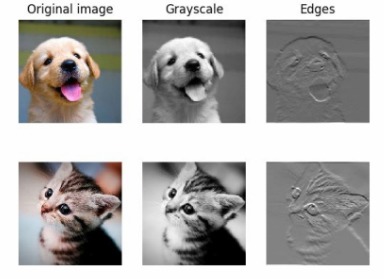
\includegraphics[width=.7\textwidth]{fig/2018-05-03-21-17-51.png}
\end{figure}

出现梯度检查(1 pnt) 

\begin{figure}[h]
	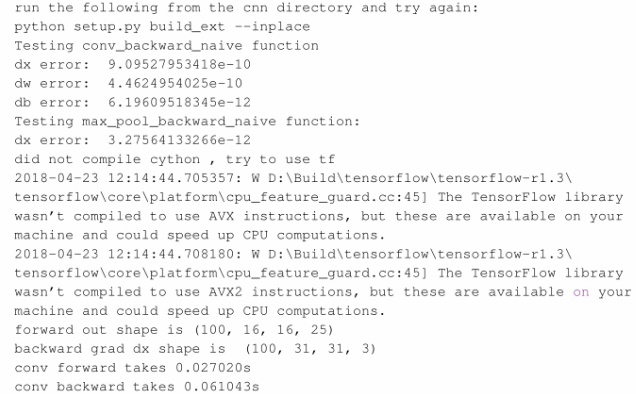
\includegraphics[width=.65\textwidth]{fig/2018-05-03-21-19-49.png}
\end{figure}

(2) 出现loss曲线或准确率曲线 0.5 pnt 

出现滤波器的可视化 1 pnt

\begin{figure}[h]
	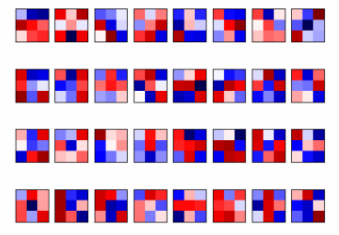
\includegraphics[width=.5\textwidth]{fig/2018-05-03-21-26-12.png}
\end{figure}

出现feature map的可视化 1 pnt

\begin{figure}[h]
	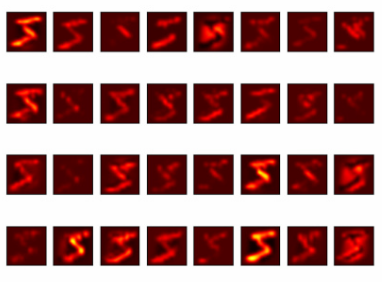
\includegraphics[width=.5\textwidth]{fig/2018-05-03-21-25-41.png}
\end{figure}

对embedding降维可视化,观察 separable 1 pnt 

\begin{figure}[h]
	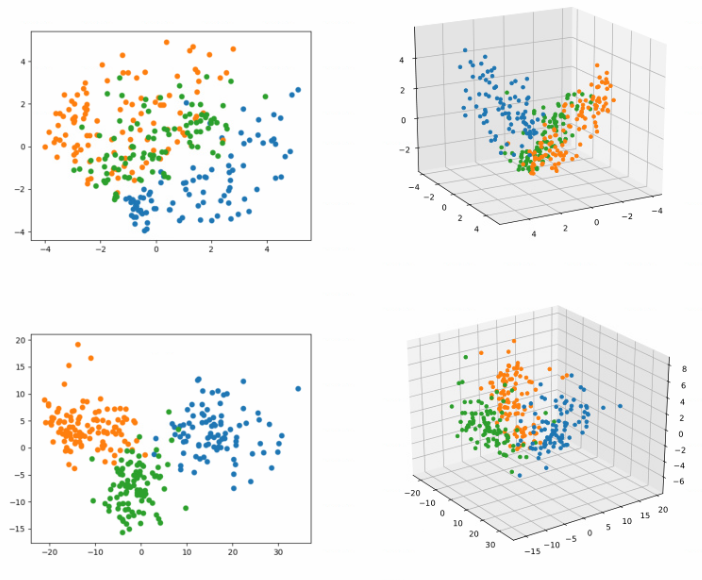
\includegraphics[width=.9\textwidth]{fig/2018-05-03-21-26-51.png}
\end{figure}

其他合理的可视化 1 pnt 

(3) 由于mnist数据集比较简单,可能使用新的模块不能体现出很好的效果。比如batchnormlize可能(由于过拟合)反而效果变差也是有可能的。做过实验给出分析即可。1 pnt 每个实验

(4) im2col解释 0.5 pnt, 解释为什么fast layer快 0.5 pnt,解释卷积为什么不用fft 0.5 pnt。 

具体为什么,可能是因为对小的卷积核,矩阵相乘比较快,对大的卷积核fft比较快?可能是复数运算对内存和计算复杂度的要求?

\end{document}

